Devido a grande quantidade de projetos desenvolvidos em paralelo no Campus Gama da Universidade de Brasília, e a desinformação a respeito do processo colaborativo em relação a estes, a empresa júnior Eletrojun foi motivada a iniciação do projeto de Compartilhamento e Gerência de projetos, com a intenção de integrar os alunos da universidade, de modo que corroborem na produção e conclusão de projetos, incentivando ainda a divulgação dos mesmos.

O objetivo desta proposta é alcançar um nível avançado e organizado de produção e controle de projetos, concentrando ainda as propostas de projeto e os projetos em andamento em uma plataforma acessível a todos os estudantes que por ventura tenham interesse em ingressar e colaborar com projetos, proporcionando desta forma uma maior completude da aplicação prática dos conhecimentos acadêmicos.

A fim de solucionar tal defasagem do âmbito de controle, criação e colaboração de projetos, a Eletrojun, sob a liderança da estudante Mônica Damasceno, iniciou a produção de um software para esta finalidade. Porém, esta produção foi interrompida ainda em sua fase inicial.

Neste cenário, se faz necessária a refatoração do produto produzido até o momento, de forma a corresponder de forma coerente às necessidades que o cliente expressa para que solucione o problema objetivo.

\section {Problema}

De forma a se conseguir traçar todos os sub-problemas e o problema raiz que a solução proposta deveria sanar, foi elaborado pela equipe de Engenharia de Requisitos, juntamente com o cliente, um diagrama de FishBone, traçando as dificuldades de produção, financeira, de instalações, divulgação, pessoas e organização, que apresentaram-se como as maiores colaboradoras para o principal problema, caracterizado pela Dificuldade no desenvolvimento coletivo de projetos. Tal diagrama é explicitado na (Figura \ref{img:problema}).


\FloatBarrier
\begin{figure}[!htpd]
		\centering
		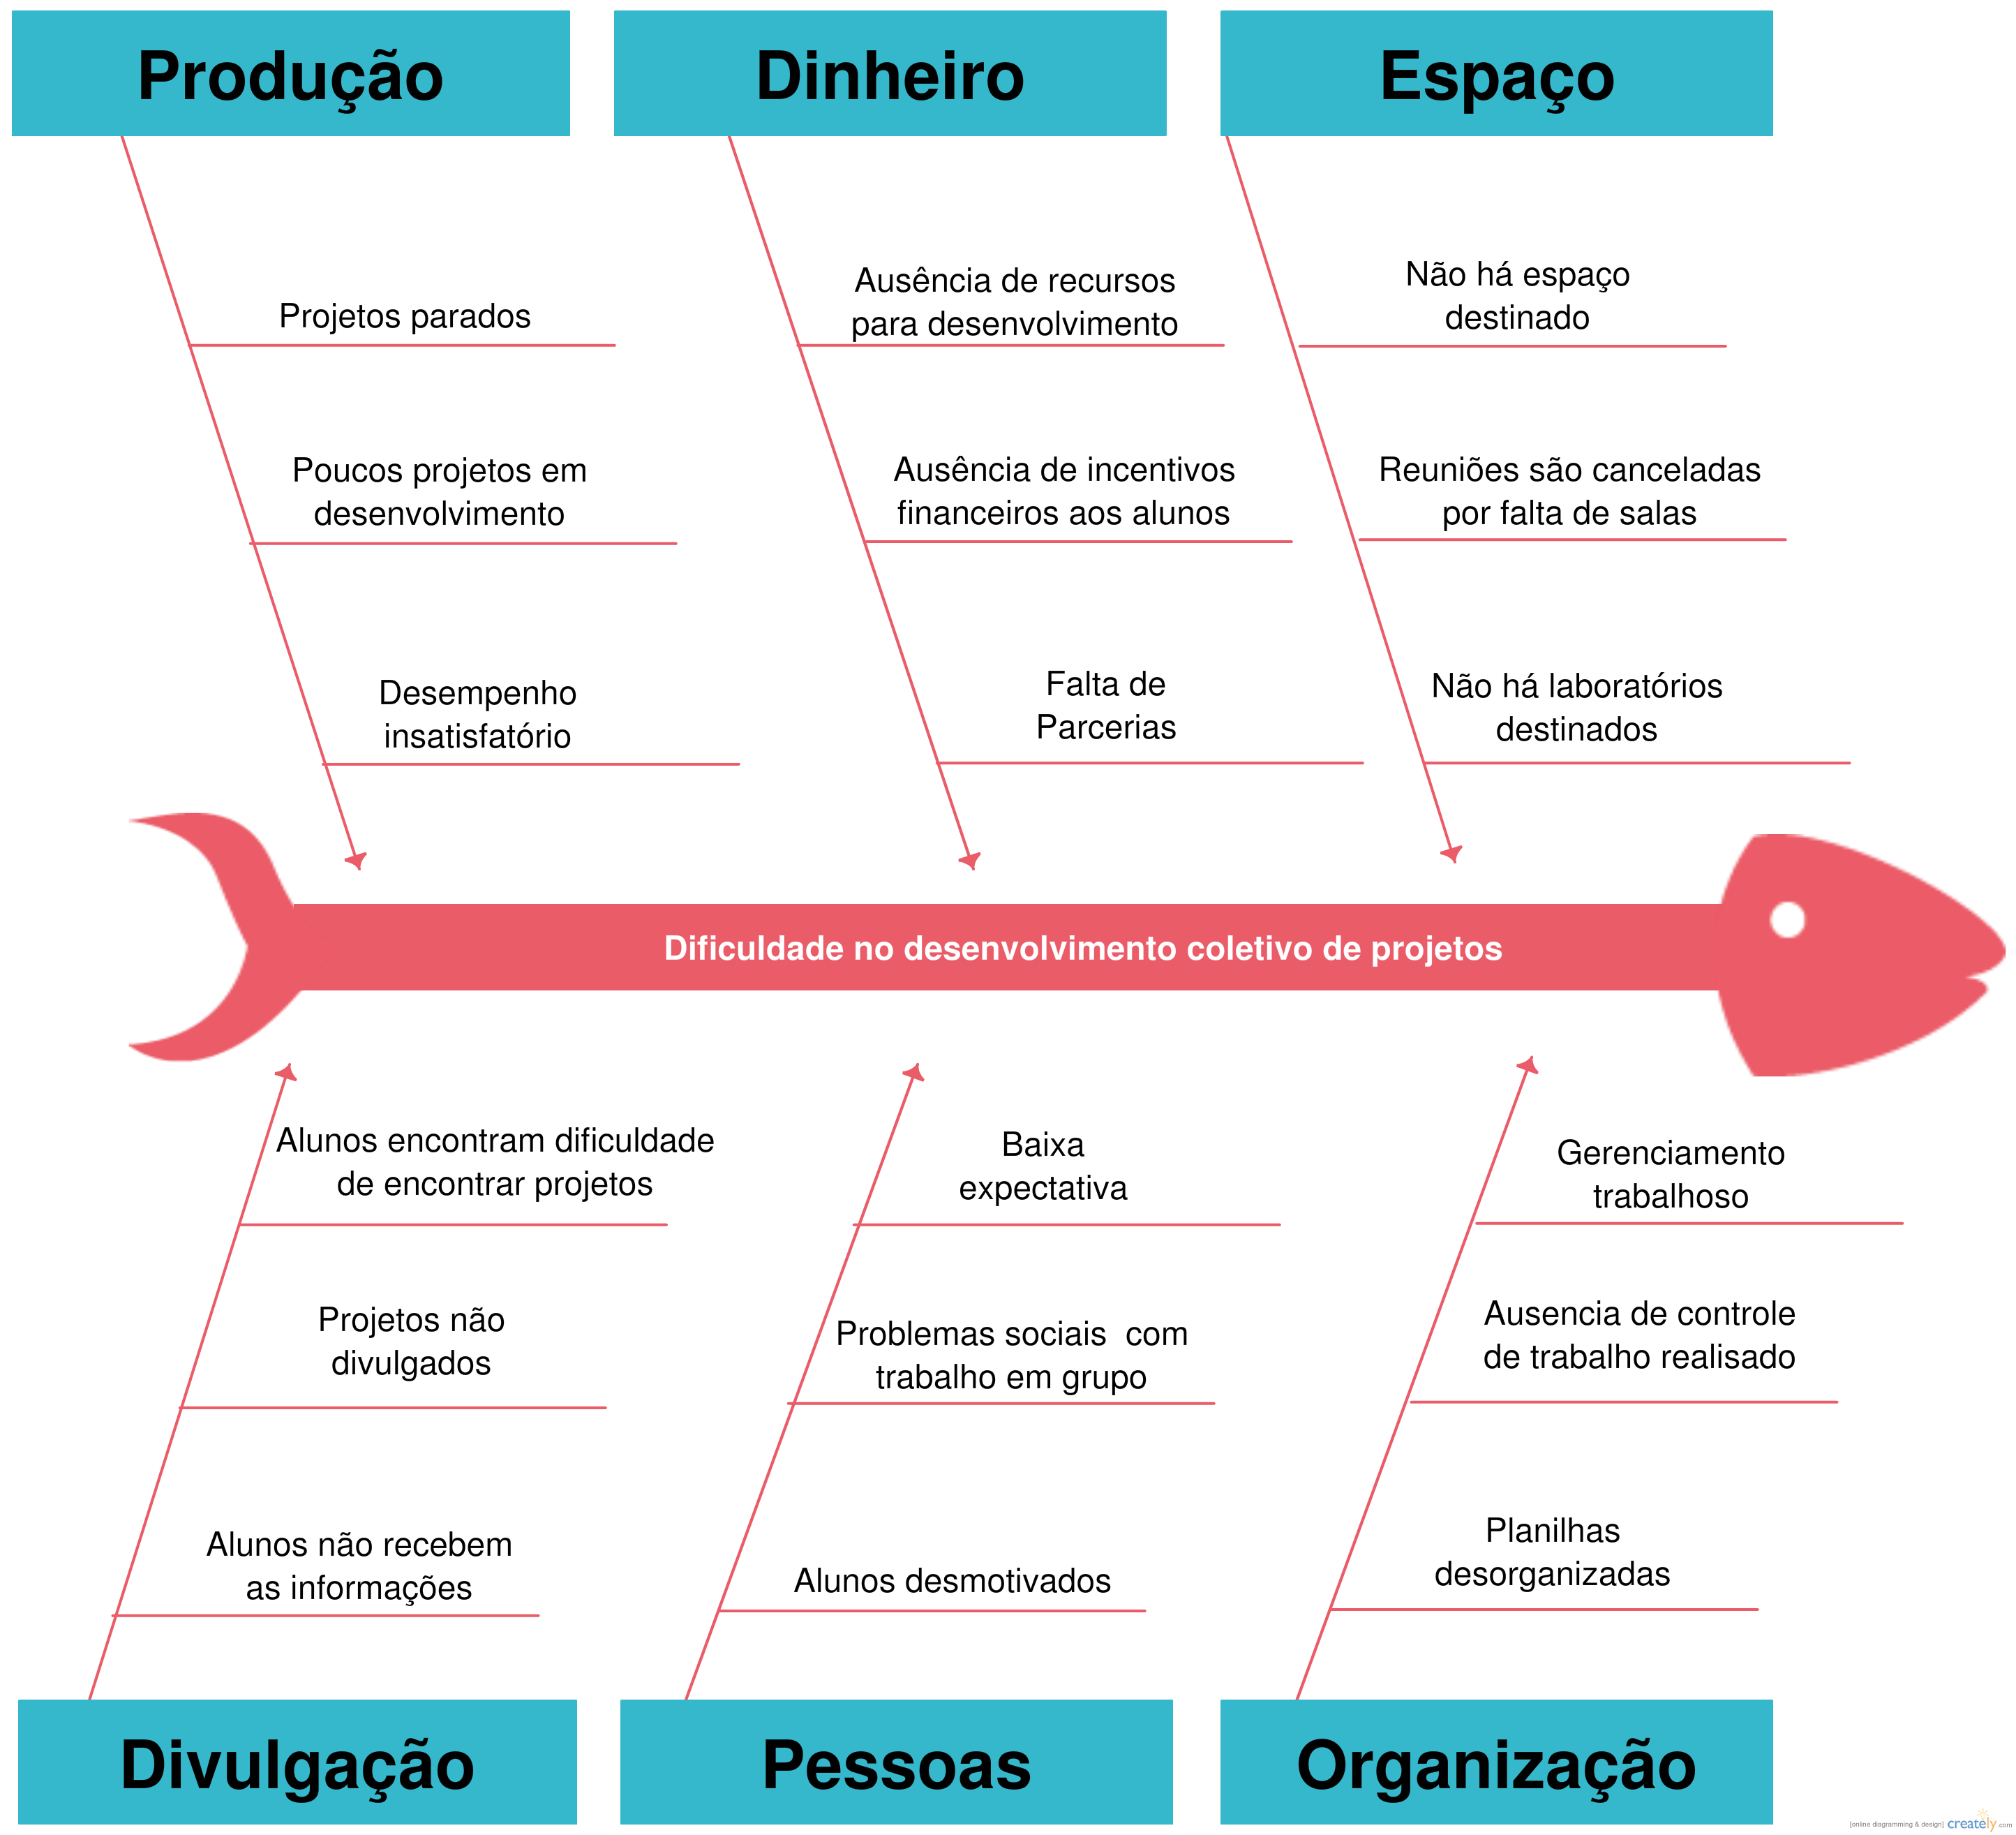
\includegraphics[scale=0.15]{figuras/problema}
		\label{img:problema}
		\caption{Diagrama de FishBone}
\end{figure}
\FloatBarrier

\section {Solução}

Foi proposta a solução de refatoração e evolução da plataforma iniciada, corrigindo problemas estruturais, funcionais e conflitos de requisitos identificados.Além de organizar sua produção, fazendo com que esta plataforma, em sua completude, permita a criação e administração de projetos de forma colaborativa, a fim de que os usuários possam evoluir seus projetos distribuindo tarefas aos colaboradores, com funcionalidade de premiação por colaborações e ranking de projetos.

Esta deve suportar ainda uma plataforma de chat entre os usuários, permitindo a interação entre estes, além de mecanismos para personalização de configurações da plataforma na página do usuário. A solução também conta com o contexto administrativo da plataforma, onde se tem um controle dos projetos e usuários cadastrados, concedido ao(s) administrador(es) da plataforma.
